\newpage
\subsubsection{Model}
Viene di seguito riportato il diagramma delle classi del package model.
\begin{figure}[H]
\centering
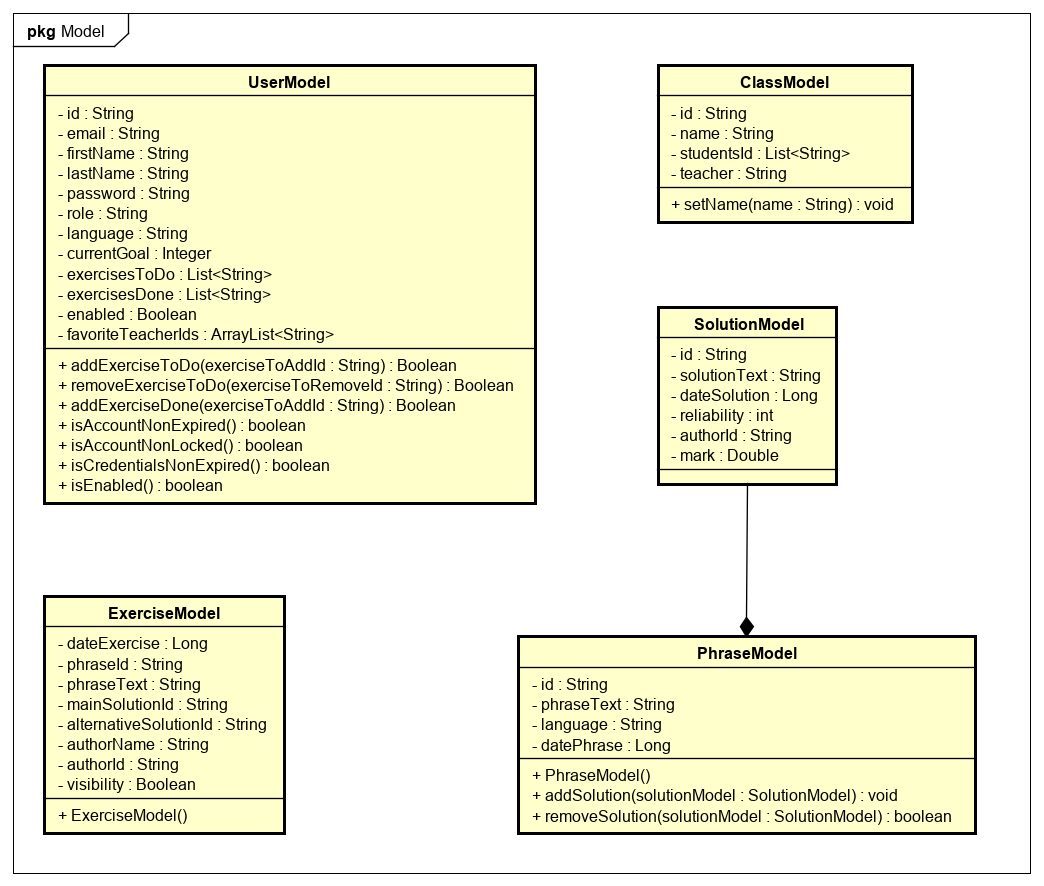
\includegraphics[width=17cm, keepaspectratio]{img/model.png} 
\caption{Model}
\end{figure}
\newpage

\subsubsection{Controller e service}
Viene di seguito riportato il diagramma delle classi di package controller e service.
\begin{figure}[H]
\centering
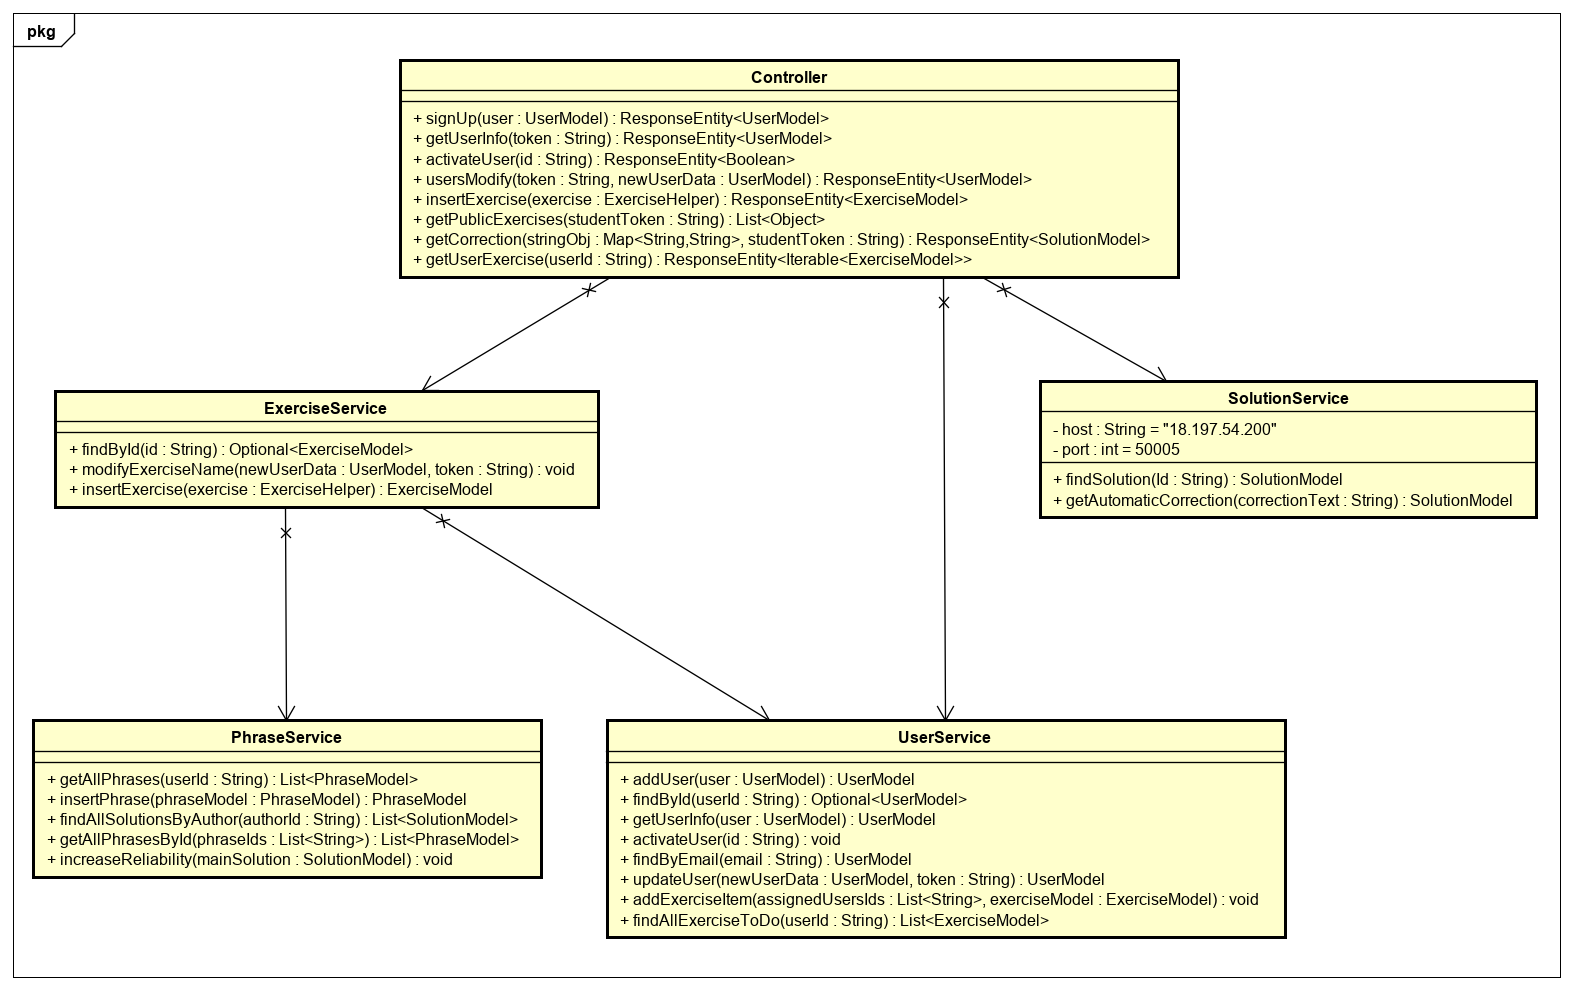
\includegraphics[width=17cm, keepaspectratio]{img/Controller-service.png} 
\caption{Controller e Service}
\end{figure}

\subsubsection{View}
Viene di seguito riportato il diagramma delle classi di package della view.
\begin{figure}[H]
\centering
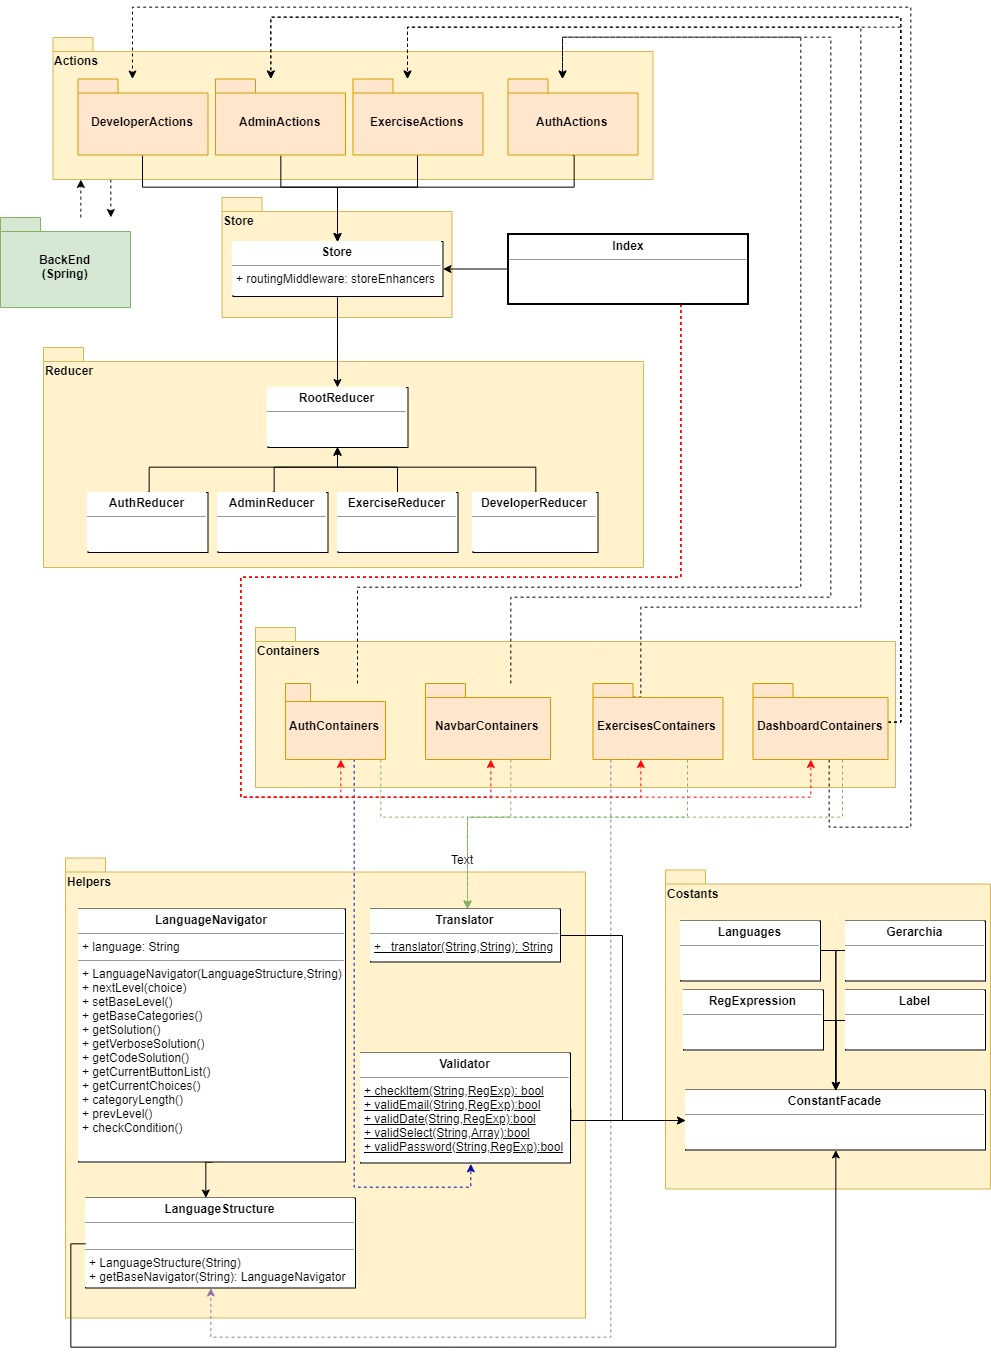
\includegraphics[width=17cm, keepaspectratio]{img/view.jpg} 
\caption{View}
\end{figure}
\newpage
\subsubsection{Service e repository}
Viene di seguito riportato il diagramma delle classi di package service e repository.
\begin{figure}[H]
\centering
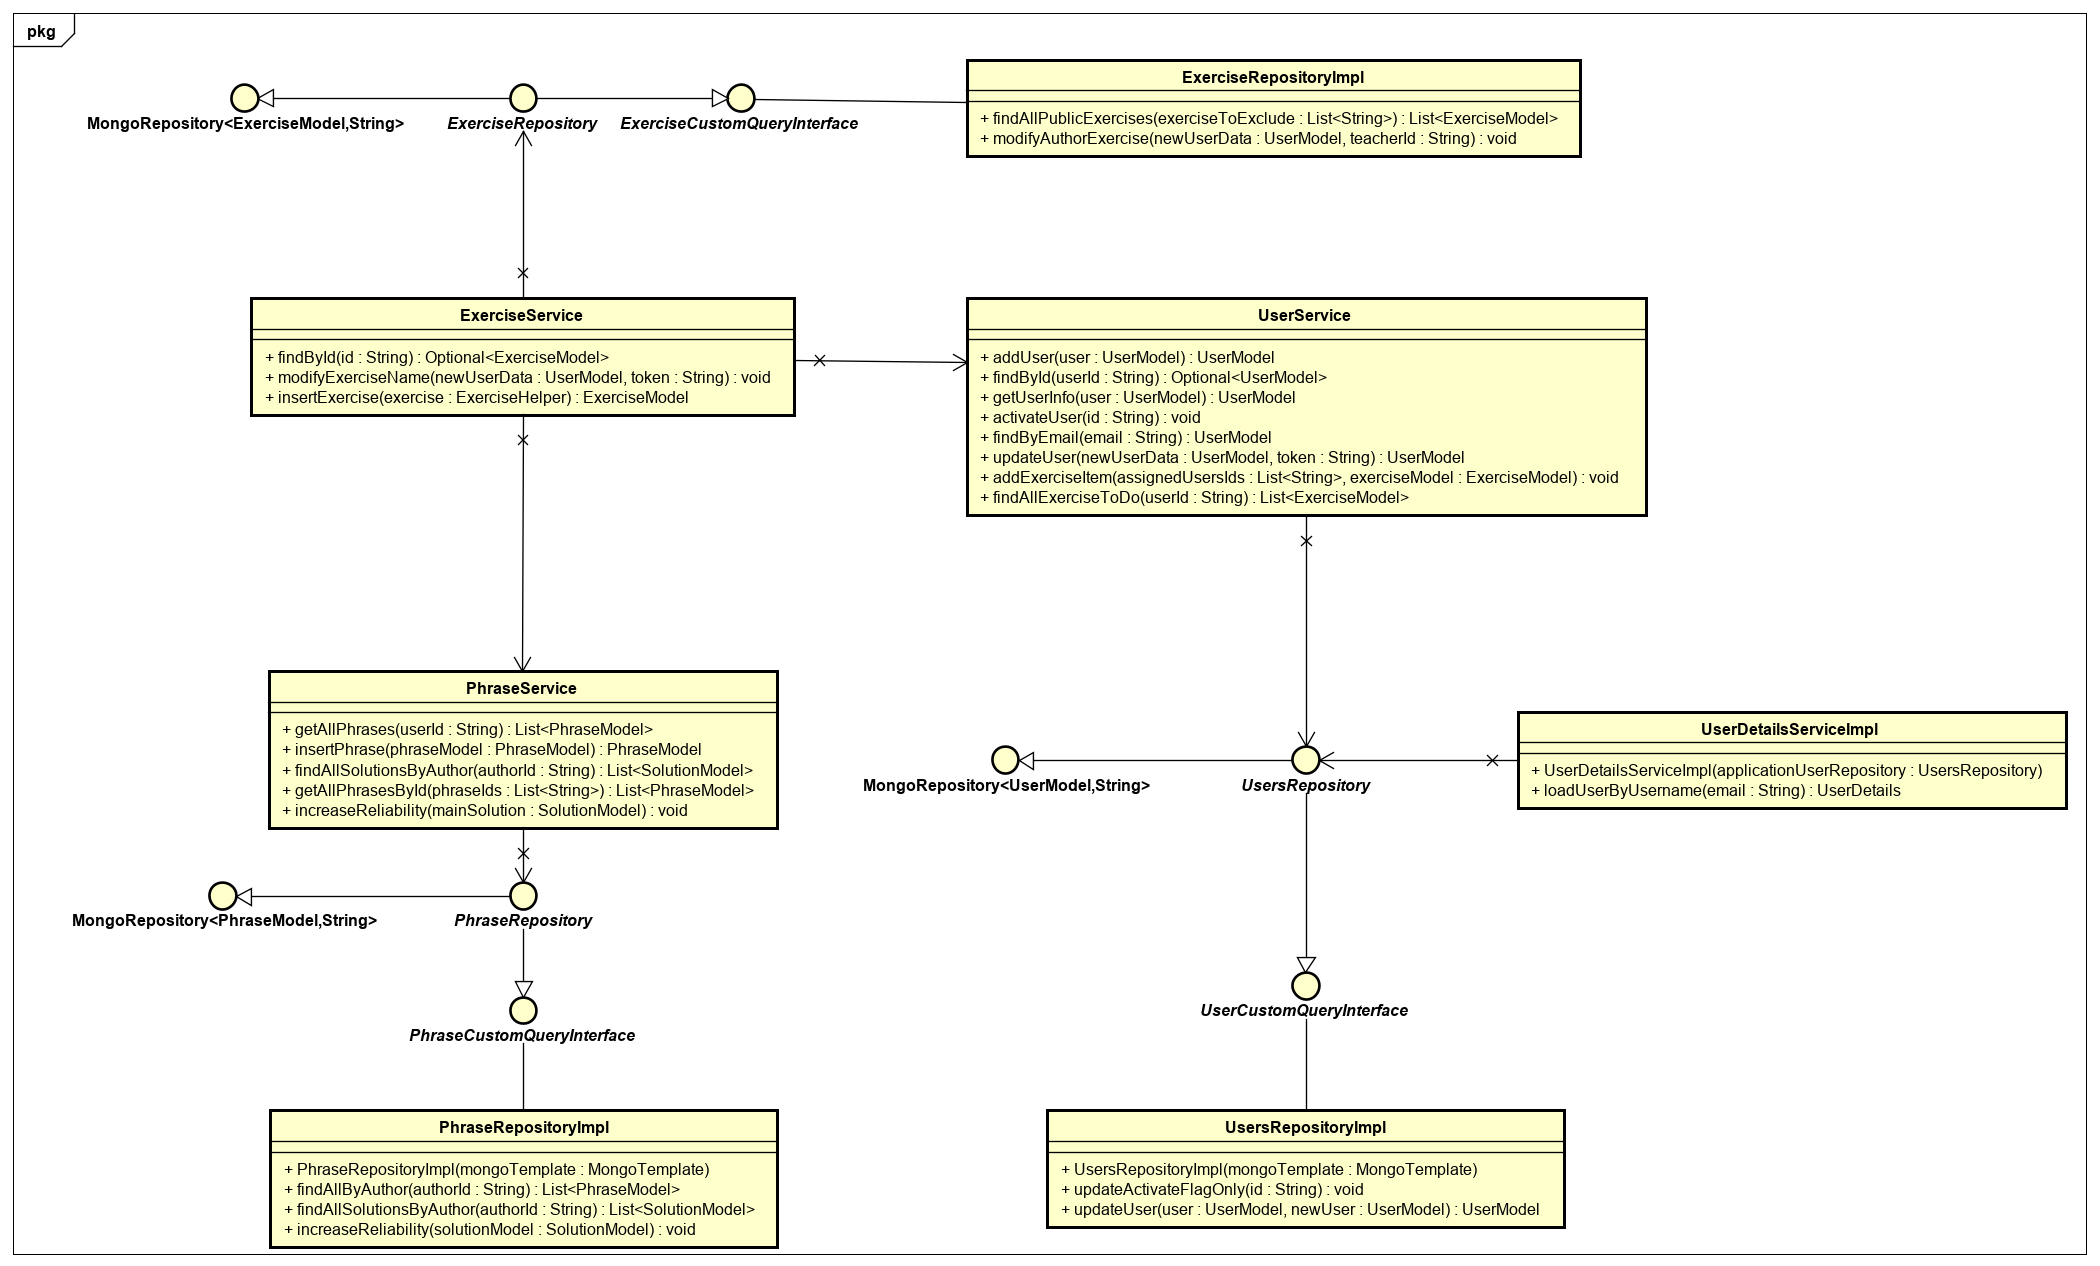
\includegraphics[width=17cm, keepaspectratio]{img/Service-repository.png} 
\caption{Service e Repository}
\end{figure}

